\begin{frame}[fragile]
\frametitle{The Limits of Parametricity}
\begin{block}{monomorphic signature}
\begin{lstlisting}[style=haskell]
[Int] -> [Int]
\end{lstlisting}
From the \emph{\textbf{monomorphic} type}, what does this function do?
\end{block}
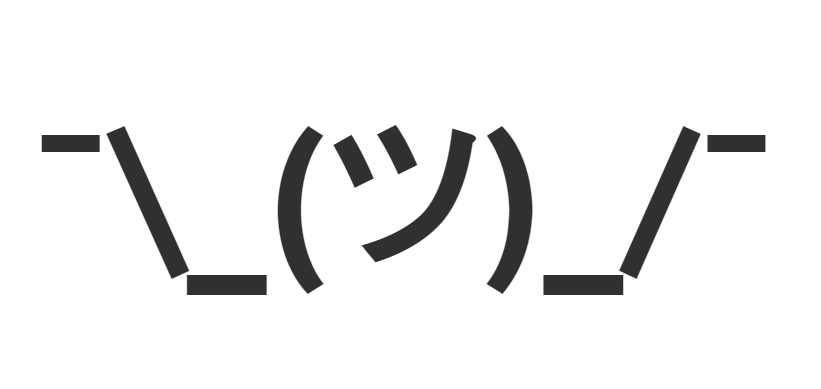
\includegraphics[width=0.2\textwidth]{image/shrug.png}
\end{frame}

\begin{frame}[fragile]
\frametitle{The Limits of Parametricity}
\begin{block}{theorems as types}
\begin{lstlisting}[style=csharp]
[a] -> [a]
\end{lstlisting}
From the \emph{\textbf{polymorphic} type}, what does this function do?
\end{block}
\large{\textbf{Theorem: all elements in the result appear in the input.}}

\tiny{How do we narrow down to disambiguity? How do we make up for this shortcoming?}
\end{frame}

\begin{frame}[fragile]
\frametitle{The Limits of Parametricity}
\begin{block}{theorems as types}
\begin{lstlisting}[style=csharp]
[a] -> [a]
\end{lstlisting}
\end{block}
We know a lot about what it does not do
\end{frame}

\begin{frame}[fragile]
\frametitle{The Limits of Parametricity}
\begin{block}{theorems as types}
\begin{lstlisting}[style=csharp]
[a] -> [a]
\end{lstlisting}
\end{block}
\emph{but we don't necessarily know exactly what it does do}
\end{frame}

\begin{frame}[fragile]
\frametitle{The Limits of Parametricity}
\begin{block}{We could}
\begin{itemize}
  \item<1-> write comments above the function

            \lstinline[style=csharp]{/* This function twiddles the database to twoddle out the twip twop */}

            \textbf{OR}
  \item<2-> write \emph{true} machine-checkable statements about the function
\end{itemize}
\end{block}
\end{frame}

\begin{frame}[fragile]
\frametitle{The Limits of Parametricity}
\begin{block}{what does this function do?}
\lstinputlisting[style=haskell]{source/reverse-with-tests.hs}
\end{block}
\end{frame}

\begin{frame}[fragile]
\frametitle{The Limits of Parametricity}
\begin{block}{what does this function do?}
\lstinputlisting[style=csharp,mathescape]{source/reverse-with-tests.cs}
\end{block}
\end{frame}

\begin{frame}[fragile]
\frametitle{The Limits of Parametricity}
\begin{block}{another example (Haskell)}
\begin{lstlisting}[style=haskell,mathescape]
flatMap :: (a -> List b) -> List a -> List b
flatMap = $\ldots$
\end{lstlisting}
\end{block}
\end{frame}

\begin{frame}[fragile]
\frametitle{The Limits of Parametricity}
\begin{block}{another example (C\#)}
\begin{lstlisting}[style=csharp,mathescape]
List<B> SelectMany<A, B>(this List<A>, Func<A, List<B>>) {
  $\ldots$
}
\end{lstlisting}
\end{block}
\end{frame}

\begin{frame}[fragile]
\frametitle{The Limits of Parametricity}
\begin{block}{another example}
\begin{lstlisting}[style=haskell,mathescape]
flatMap :: (a -> List b) -> List a -> List b
flatMap = $\ldots$
\end{lstlisting}
\begin{lstlisting}[style=csharp,mathescape]
List<B> SelectMany<A, B>(this List<A>, Func<A, List<B>>) {
  $\ldots$
}
\end{lstlisting}
\end{block}
\begin{itemize}
  \item If the input list is empty, so is the result
  \item Every \lstinline{(b)} in the result came from application of the given function
\end{itemize}
\end{frame}

\begin{frame}[fragile]
\frametitle{Once-inhabitance}
\begin{block}{sometimes tests are unnecessary}
\begin{lstlisting}[style=haskell]
f :: a -> a
\end{lstlisting}
\end{block}
\end{frame}

\begin{frame}[fragile]
\frametitle{Once-inhabitance}
\begin{block}{sometimes tests are unnecessary}
\begin{lstlisting}[style=haskell]
g :: Functor f => y -> f x -> f y
\end{lstlisting}
\end{block}
\emph{We already know that}
\begin{lstlisting}[style=haskell,mathescape]
$\lambda$> g "hi" [1,2,3]
["hi","hi","hi"]
\end{lstlisting}
\end{frame}

\begin{frame}[fragile]
\frametitle{Once-inhabitance}
\begin{block}{sometimes tests are \textbf{almost} unnecessary}
\begin{lstlisting}[style=haskell]
h :: a -> a -> a
\end{lstlisting}
\begin{lstlisting}[style=csharp]
A h<A>(A a1, A a2)
\end{lstlisting}
\end{block}
\end{frame}

\begin{frame}[fragile]
\frametitle{Once-inhabitance}
\begin{block}{sometimes tests are \textbf{almost} unnecessary}
\begin{lstlisting}[style=haskell]
h :: a -> a -> a
\end{lstlisting}
\begin{lstlisting}[style=csharp]
A h<A>(A a1, A a2)
\end{lstlisting}

\end{block}
\begin{lstlisting}[style=haskell,mathescape]
$\lambda$> h 7 8
7
\end{lstlisting}
\begin{lstlisting}[style=csharp]
csharp> h(7, 8)
7
\end{lstlisting}
\emph{We now know \textbf{precisely} what this function does}
\end{frame}

\begin{frame}[fragile]
\frametitle{Parametricity}
\begin{block}{non-trivial example}
\begin{lstlisting}[style=haskell]
both ::
  (Applicative f, Bitraversable r) =>
  (a -> f b) -> r a a -> f (r b b)
\end{lstlisting}
\end{block}
\begin{center}
What might this function do and what are the limitations of reasoning?
\end{center}
\end{frame}

\begin{frame}[fragile]
\frametitle{Parametricity}
\begin{block}{and so on}
\begin{lstlisting}[style=haskell]
point :: Store a b -> b

data Store a b = Store (a -> b) b
\end{lstlisting}
\end{block}
\end{frame}

\begin{frame}[fragile]
\frametitle{Parametricity}
\begin{block}{and on}
\begin{lstlisting}[style=haskell]
_1 :: Lens (a, x) (b, x) a b
\end{lstlisting}
\end{block}
\end{frame}
